\documentclass{article}


\include{stddefs}
\include{imodefs}

\begin{document}



\chapterno{8}
\chapter{The Hessian}

In Chapter \ref{chapter:convexfunctions} we exploited the second derivative
$f''(x)$ of a one variable real function $f:(a, b) \rightarrow \RR$ to analyze
convexity along with local minima and maxima.

In this chapter we introduce an analogue of the second derivative for real functions $f:\RR^n\rightarrow \RR$ of
several variables. This will be an $n\times n$ matrix. The important notion of a matrix
being positive (semi-) definite introduced in Section \ref{Sectionsymmat} will now
make its appearance.

\section{Introduction}

In Section \ref{section:Taylor} the Taylor expansion for a one variable differentiable
function $f:\RR\rightarrow \RR$ centered a $x_0$ with step size
$h  = x - x_0$ was introduced as
\begin{equation}\label{taylor}
f(x_0 + h) = f(x_0) + f'(x_0) h + \frac{1}{2} f''(x_0) h^2 + \cdots
\end{equation}

Recall that the second derivative $f''(x_0)$ contains a
wealth of information about the function. Especially if $f'(x_0) = 0$,
then we might glean from $f''(x_0)$ if $x_0$ is a local maximum or
minimum or none of these (see Theorem \ref{derconv} and review Exercise \ref{exderconv}).

We also noticed that gradient descent did not work so well only
descending along the gradient. We need to take the second
derivative into account to get a more detailed picture of the
function.

\section{Several variables}

Our main character is a differentiable function $F:\RR^n\rightarrow \RR$ in
several variables. We already know that
$$
F(x_0 + h) = F(x_0) + \nabla F(x_0) h + \epsilon(h) \abs{h},
$$
where $x_0$ and $h$ are vectors in $\RR^n$ (as opposed to the good old
numbers in \eqref{taylor}). Take a look back at Definition \ref{diffdef} for
the general definition of differentiability.

We wish to have an analogue of the Taylor expansion in \eqref{taylor} for
such a function of several variables. To this end we introduce the function
$g:\RR\rightarrow \RR$ given by
\begin{equation}\label{onedimg}
g(t) = F(x_0 + t h).
\end{equation}
Notice that
$$
g(t) = (F\circ A)(t),
$$
where $A: \RR\rightarrow \RR^n$ is the function given by $A(t) = x_0 + t h$. In particular
we get
\begin{equation}\label{chrule1}
g'(t) = F'(x_0 + t h) h = \nabla F(x_0 + t h) h
\end{equation}
by using the chain rule (see Theorem \ref{chainrule}).

\beginshex
Explain how the chain rule is applied to get \eqref{chrule1}.
\endshex

The derivative $g'(t)$ is also composed of several functions and again we may
compute $g''(t)$ by using the chain rule:
\begin{align}
  g''(t) &= (C\circ B \circ A)'(t)\\
        &= (C\circ B)'(A(t)) A'(t) \\
        &= C'(B(A(t))) B'(A(t)) A'(t),
\end{align}
where $B: \RR^n\rightarrow \RR^n$ is defined by
$$
B(v) = \nabla F(v)^T
$$
and $C:\RR^n \rightarrow \RR$ by
$$
C(v) = v^T h.
$$

\begin{definition}[emph]

The \emph{Hessian matrix} of $F$ at the point
$x\in \RR^n$ is defined by

\begin{equation*}
  \nabla^2 F(x) :=
  \begin{pmatrix}
    \dfrac{ \partial^2 F}{ \partial x_1 \partial x_1}(x) &
    \cdots & \dfrac{ \partial^2 F}{ \partial x_1 \partial
      x_n}(x)
    \\
    \vdots & \ddots & \vdots
    \\
    \dfrac{ \partial^2 F}{ \partial x_n \partial x_1}(x) &
    \cdots & \dfrac{\partial^2 F}{ \partial x_n\partial
      x_n}(x)
  \end{pmatrix}
  .

\end{equation*}
\end{definition}



A very important observation is that $\nabla^2 F(x)$ above is a
symmetric matrix. Again, you should review what this means by clicking
back to Section \ref{Sectionsymmat}.

\beginshex
Why is the Hessian matrix symmetric?
\endshex

\begin{example}\label{sagegradhess}
  Suppose that $f: \RR^2\rightarrow \RR$ is given by
  $$
  f(x, y) = \sin(x y) + x^2 y^2 + y.
  $$
  Then the gradient
  $$
  \nabla f = \left(\frac{\partial f}{\partial x}, \frac{\partial f}{\partial y} \right)
  $$
  and the Hessian

  $$
  \nabla^2 f =
  \begin{pmatrix}
    \dfrac{\partial^2 f}{\partial x^2} & \dfrac{\partial^2 f}{\partial x \partial y} \\
    \\
    \dfrac{\partial^2 f}{\partial y \partial x} & \dfrac{\partial^2 f}{\partial y^2}
  \end{pmatrix}
  $$
  of $f$ are computed in the Sage window below.

  \begin{sage}
x, y = var('x, y')
f = sin(x*y) + x^2*y^2 + y
print("gradient = ", f.gradient())
print("Hessian = ", f.hessian())
  \end{sage}

See the \url{further documentation}{http://doc.sagemath.org/html/en/reference/calculus/sage/calculus/functions.html} for Calculus functions in Sage.
\end{example}


  
\beginshex
Verify (just this once) by hand the computations done by Sage in Example \ref{sagegradhess}.

Also, experiment with a few other functions in the Sage window and compute their
Hessians.
\endshex



By applying Proposition \ref{proppd} it is not too hard to see that the Hessian
matrix fits nicely into the framework above, since
\begin{equation}\label{exhess}
B'(v) = \nabla^2 F(v).
\end{equation}

The full application of the chain rule then gives
\begin{equation}\label{chrule2}
g''(t) = h^T \nabla^2 F(x_0 + t h) h.
\end{equation}


\beginshex
Give a detailed explanation as to why \eqref{exhess} holds.
\endshex


\section{Newton's method for finding critical points}

We may use Newton's method for computing critical points for a function
$F:\RR^n\rightarrow \RR$ of several variables. Recall that a
critical point is a point $x_0\in \RR^n$ with $\nabla F(x_0) = 0$.
By \eqref{onestepmultnewt} and \eqref{exhess} the computation in Newton's method becomes
\begin{equation}\label{newthess}
x_1 = x_0 - \left(\nabla^2 F(x_0)\right)^{-1} \nabla F(x_0).
\end{equation}
In practice 
the (inverse) Hessian appearing in \eqref{newthess} is often a heavy
computational burden. This leads to the socalled
\url{quasi-Newton methods}{https://en.wikipedia.org/wiki/Quasi-Newton_method}, where
the inverse Hessian in \eqref{newthess} is replaced by other matrices. 


\begin{example}\label{Exbadlogist}
We will return to the logistic regression in Example \ref{challengerexample} about the
Challenger disaster. Here we sought to maximize the function
  \begin{equation}\label{logtwo}
  \ell(\alpha, \beta) = \sum_{i=1}^m E_i (\alpha + \beta x_i) - \log(1 + e^{\alpha + \beta x_i}).
  \end{equation}

In order to employ Newton's method we compute the gradient and the Hessian of \eqref{logtwo}
\begin{align}\label{hesslogist}
  \frac{\partial \ell}{\partial \alpha} &= \sum_{i=1}^m E_i - \sigma(\alpha + \beta x_i)\\
  \frac{\partial \ell}{\partial \beta} &= \sum_{i=1}^m E_i x_i - x_ i\sigma(\alpha + \beta x_i)\\
  \frac{\partial^2 \ell}{\partial \alpha^2} &= \sum_{i=1}^m - \sigma'(\alpha + \beta x_i)\\
  \frac{\partial^2 \ell}{\partial \beta \partial \alpha} &= \sum_{i=1}^m -\sigma'(\alpha + \beta x_i) x_i\\
  \frac{\partial^2 \ell}{\partial \beta^2} &= \sum_{i=1}^m - \sigma'(\alpha + \beta x_i) x_i^2,
\end{align}
where
$$
\sigma(t) = \frac{1}{1 + e^{-t}}
$$
is the sigmoid function.

Notice the potential problem in using Newton's method here: the formula for
the second order derivatives in \eqref{hesslogist} show that if the $\alpha +\beta x_i$ are just mildly big, say $\geq 50$, then
the Hessian is extremely close to the zero matrix and therefore Sage considers it non-invertible and
\eqref{newthess} fails.

In the code below we have nudged the initial vector so that it works, but you
can easily set other values and see its failure. Optimization is not just mathematics, it also calls
for some good (engineering) implementation skills (see for example details on the
\url{quasi Newton algorithms}{https://en.wikipedia.org/wiki/Quasi-Newton_method}).

In the instance below we do, however, get a gradient that is pratically $(0, 0)$.
  
\begin{hideinbutton}{Code for Newton's method}
\begin{sage}
x0 = [11,-0.2] 
noofits = 10
  

x = [53.0, 56.0, 57.0, 63.0, 66.0, 67.0, 67.0, 67.0, 68.0, 69.0, 70.0, 70.0, 70.0, 70.0, 72.0, 73.0, 75.0, 75.0, 76.0, 76.0, 78.0, 79.0, 80.0, 81.0]
E = [1.0, 1.0, 1.0, 0.0, 0.0, 0.0, 0.0, 0.0, 0.0, 0.0, 0.0, 1.0, 0.0, 1.0, 0.0, 0.0, 0.0, 1.0, 0.0, 0.0, 0.0, 0.0, 0.0, 0.0]

Es = sum(E)
Exs = sum(u*v for (u, v) in zip(x, E))
    
def sigmoid(a, b, x):
  s = 1/(1 + exp(-a - b*x))
  return s.n()

def sigmoidm(a, b, x):
  s = sigmoid(a, b, x)
  return s*(1-s)
      
def gradient(v):
  a = v[0]
  b = v[1]
  return vector((Es - sum(sigmoid(a, b, t) for t in x), Exs - sum(t*sigmoid(a, b, t) for t in x)))
    
def hessian(v):
  a = v[0]
  b = v[1]
  h11 = - sum(sigmoidm(a, b, t) for t in x)
  h12 = - sum(sigmoidm(a, b, t)*t for t in x)
  h22 = - sum(sigmoidm(a, b, t)*t*t for t in x)
  return matrix([[h11, h12], [h12, h22]])

def newtonstep(v0):
  d = gradient(v0)
  h = hessian(v0)
  return v0 - h.inverse()*d

v = vector(x0)  
for k in range(noofits):
  print(v)
  v = newtonstep(v)

print("x0 = ", x0)
print("Number of Newton iterations =  ", noofits)
print("Predicted maximal point =  ", v)

alpha = v[0]
beta = v[1]

print("Gradient at predicted maximal point = ", gradient(v))
print("Predicted probability of failure at 31F = ", sigmoid(alpha, beta, 31))
\end{sage} 
\end{hideinbutton}
\end{example}


\subsection{Transforming data for better numerical performance}

The numerical problems with Newton's method in Example \ref{Exbadlogist} can be prevented by transforming the input data.
It makes sense to transform data from large numbers to
smaller numbers around $0$. There is a rather standard way of doing this.

Suppose in logistic regression we have a set of data
\begin{equation}\label{datapts}
x_1, x_2, \dots, x_n
\end{equation}
associated with outcomes $E_1, \dots, E_n$. Then the function
  $$
  \ell(\alpha, \beta) = \sum_{i=1}^m E_i (\alpha + \beta x_i) - \log(1 + e^{\alpha + \beta x_i}).
  $$
  from Example \ref{exlogist} becomes much more manageable if we first
  transform the data according to
  $$
  x'_i = \frac{x_i - \overline{x}}{\sigma} 
  $$
  and instead optimize the function
  $$
  \ell'(\alpha, \beta) = \sum_{i=1}^m E_i (\alpha + \beta x'_i) - \log(1 + e^{\alpha + \beta x'_i}).
  $$
  Here
  $$
  \overline{x} = \frac{x_1 + x_2 + \cdots + x_n}{n}
  $$
  is the mean value and
  $$
  \sigma^2 = \frac{(x_1 - \overline{x})^2 + (x_2 - \overline{x})^2 + \cdots + (x_n - \overline{x})^2}{n}
  $$
  the variance of the data in \eqref{datapts}.

  
  Now if $\alpha'$ and $\beta'$ is an optimum for $\ell'$, then
  \begin{align}\label{transformtrick}
    \alpha &= \alpha' - \frac{\overline{x}}{\sigma} \beta'\\
    \beta &= \frac{\beta'}{\sigma}
  \end{align}
  is an optimum for $\ell$, since
  $$
  \ell'(\alpha, \beta) = \ell\left(\alpha - \beta \frac{\overline{x}}{\sigma}, \frac{\beta}{\sigma}\right).
  $$

\beginshex
Why is the claim/trick alluded to in \eqref{transformtrick} true?

Below is a snippet of Sage code implementing the trick in \eqref{transformtrick}.
The function \texttt{test} takes as input \texttt{x0} (an initial vector like \texttt{[0,0]}) and
\texttt{noofits} (the number of iterations of Newton's method). You execute this in the Sage
window by adding for example
\begin{code}
  test([0,0], 10)
\end{code}
and then pressing \texttt{Compute}.

Experiment and compare with the official output from Example \ref{challengerexample}. Also, compute
the gradient of the output below for the original non-transformed problem.

\begin{hideinbutton}{Transformed code}
\begin{sage}
x = [53.0, 56.0, 57.0, 63.0, 66.0, 67.0, 67.0, 67.0, 68.0, 69.0, 70.0, 70.0, 70.0, 70.0, 72.0, 73.0, 75.0, 75.0, 76.0, 76.0, 78.0, 79.0, 80.0, 81.0]
E = [1.0, 1.0, 1.0, 0.0, 0.0, 0.0, 0.0, 0.0, 0.0, 0.0, 0.0, 1.0, 0.0, 1.0, 0.0, 0.0, 0.0, 1.0, 0.0, 0.0, 0.0, 0.0, 0.0, 0.0]
mean = sum(x)/len(x)
std = sqrt(sum(map(lambda t: (t-mean)^2, x))/len(x))

x = list(map(lambda t: (t-mean)/std, x))


Es = sum(E)
Exs = sum(u*v for (u, v) in zip(x, E))
    
def sigmoid(a, b, x):
  s = 1/(1 + exp(-a - b*x))
  return s.n()

def sigmoidm(a, b, x):
  s = sigmoid(a, b, x)
  return s*(1-s)
      
def gradient(v):
  a = v[0]
  b = v[1]
  return vector((Es - sum(sigmoid(a, b, t) for t in x), Exs - sum(t*sigmoid(a, b, t) for t in x)))
    
def hessian(v):
  a = v[0]
  b = v[1]
  h11 = - sum(sigmoidm(a, b, t) for t in x)
  h12 = - sum(sigmoidm(a, b, t)*t for t in x)
  h22 = - sum(sigmoidm(a, b, t)*t*t for t in x)
  return matrix([[h11, h12], [h12, h22]])

def newtonstep(v0):
  d = gradient(v0)
  h = hessian(v0)
  return v0 - h.inverse()*d


def test(x0, noofits):
  v = vector(x0)  
  for k in range(noofits):
    print(v)
    v = newtonstep(v)
  print("Number of Newton iterations =  ", noofits)
  print("Predicted maximal point in transformed problem =  ", v)
  tv =   matrix([[1, -mean/std], [0, 1/std]])*v
  print("Predicted maximal point in original problem =  ", tv)


  
\end{sage}
\end{hideinbutton}
\endshex

\section{The Taylor series in several variables}

Now we are in a position to state at least the first terms in the
Taylor expansion for a differentiable function $F:\RR^n\rightarrow \RR$.
The angle of the proof is to reduce to the one-dimensional case through
the function $g(t)$ defined in \eqref{onedimg}. Here
one may prove that

\begin{equation}\label{taylorg}
g(t) = g(0) + g'(0) t + \frac{1}{2} g''(0) t^2 + \epsilon(t)t^2,
\end{equation}
where $\epsilon(0) = 0$ with $\epsilon$ continuous at $0$, much like
in the definition of differentiability except that we also include
the second derivative.

Now \eqref{taylorg} translates into

\begin{equation}\label{critminmax}
  F(x_0 + t h) = F(x_0) + \left(\nabla F(x_0) h \right) t + \frac{1}{2} \left( h^T \nabla^2 F(x_0) h \right) t^2 + \epsilon(t) t^2 
\end{equation}
by using \eqref{chrule1} and \eqref{chrule2}.

From \eqref{critminmax} one reads the following nice criterion, which may be viewed as a several variable generalization of Theorem \ref{derconv}.

\begin{theorem}[emph]\label{thmcritminmax}
  Let $x_0$ be a critical point for $F:\RR^n\rightarrow \RR$. Then
  \begin{enumerate}[(i)]
  \item
    $x_0$ is a local minimum if $\nabla^2 F(x_0)$ is positive definite.
  \item
    $x_0$ is a local maximum if $-\nabla^2 F(x_0)$ is positive definite (here we call
    $\nabla^2 F(x_0)$ negative definite).
  \item\label{thmcritminsaddle}
    $x_0$ is a \url{saddle point}{https://en.wikipedia.org/wiki/Saddle_point} if $\nabla^2 F(x_0)$ is indefinite.
  \end{enumerate}
\end{theorem}

\begin{remark}
  We need to clarify two things concerning the above theorem. 

  \begin{enumerate}[(i)]
  \item
    An $n\times n$ indefinite matrix is a symmetric matrix $A$ with the property that there exists
    $u, v\in \RR^n$ with
    \begin{align*}
      u^T A u &>0\quad\text{and}\\
      v^T A v &<0
    \end{align*}
  \item
    A saddle point $x_0$ for $F$ is defined by the existence of two vectors $u, v\in \RR^n$, such that
    \begin{align*}
      &t=0\quad \text{is a local minimum for the function}\quad f(t) = F(x_0 + t u)\\
      &t=0\quad \text{is a local maximum for the function}\quad  g(t) = F(x_0 + t v)
    \end{align*}
    as illustrated in the graphics below.

    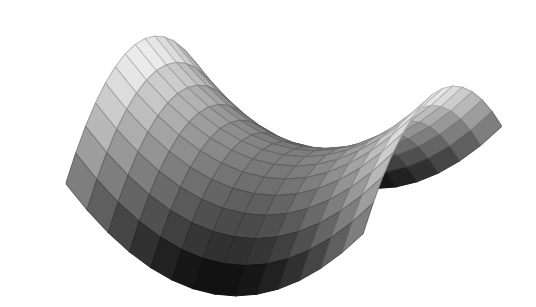
\includegraphics{saddle.png}
    \end{enumerate}
\end{remark}

\begin{example}\label{examplehesscrit}
Consider, with our new technology in Theorem \ref{thmcritminmax}, Exercise \ref{exsaddlept} once again.
Here we analyzed the point $v_0 = (0, 0)$ for the function
$$
f(x, y) = x^3 + x y + y^3
$$
and showed (by a trick) that $v_0$ is neither a local maximum nor a local minimum for $f$. The Hessian
matrix for $f(x, y)$ at $v_0$ is
$$
H = \begin{pmatrix} 0 & 1 \\ 1 & 0 \end{pmatrix}.
$$

Now
Theorem \ref{thmcritminmax}\ref{thmcritminsaddle} shows that $v_0$ is a saddle point, since
$$
\begin{pmatrix} x & y \end{pmatrix} H \begin{pmatrix} x \\ y \end{pmatrix} = 2 x y
$$ 
and
\begin{align*}
u^T H u &> 0\qquad\text{for } u = \begin{pmatrix} 1 \\ 1 \end{pmatrix}\\
v H v &< 0\qquad\text{for } v =  \begin{pmatrix} 1 \\ -1 \end{pmatrix}.
\end{align*}

\begin{sage}
x, y = var('x, y')
a = 1
plot3d(x^3 + a*x*y+ y^3, (x, -0.4, 0.4), (y, -0.4, 0.4), 
adaptive=True, color=rainbow(60, 'rgbtuple'))
\end{sage}
\end{example}

\beginshex
Try plotting the graph for \footnote{different values of \texttt{a}}{\texttt{a=4} shows the saddle point clearly.} in the Sage window in 
Example \ref{examplehesscrit}. What do you observe for the point $v_0$ with
respect to the function? Does \texttt{a} have to be a number? Could it be a symbolic
expression in the variables \texttt{x} and \texttt{y} like \texttt{a = -10*cos(x)*sin(y)}?
\endshex

\beginshex
Check the computation of the Hessian matrix $H$ in Example \ref{examplehesscrit} by showing
that the Hessian matrix for $f$  at the point $(x, y)$ is
$$
\begin{pmatrix}
6 x & 1\\
1 & 6 y
\end{pmatrix}. 
$$
\endshex

\beginshex
What about $u$ and $v$ in Example \ref{examplehesscrit}? How do they relate to the hint
given in Exercise \ref{exsaddlept}?
\endshex


\beginshex
  Give an example of a function $F:\RR^2\rightarrow \RR$ having a local minimum at
  $x_0$, where $\nabla^2 F(x_0)$ is not positive definite.
\endshex

\beginshex

The following exercise is a \texttt{sci2u} exercise from the Calculus book.

\begin{enumerate}[(i)]
\item
  The point $\left(0, \frac{\sqrt{3}}{3}\right)$ is a critical point for
  $$
  f(x, y) = x^3 + y^3 - y.
  $$
  What does Theorem \ref{thmcritminmax} say about this point?
\item
  The point $\left(\frac{1}{3}, \frac{1}{3}\right)$ is a critical point for
  $$
  f(x, y) = -x^3 -x^2 + x - y^3 + 2 y^2 - y.
  $$
  What does Theorem \ref{thmcritminmax} say about this point?
\item
  The point $(0, 1)$ is a critical point for
  $$
  f(x, y) = x^3 - x^2 + y^3 - y^2 - y.
  $$
  What does Theorem \ref{thmcritminmax} say about this point?
\end{enumerate}
\endshex
  

\beginshex
Consider the function
$$
f(x, y) = x^4 y^2 + x^2 y^4 - 3 x^2 y^2.
$$
Compute its critical points and decide on their types according to Theorem \ref{thmcritminmax}. 
Try to convince yourself that
$$
f(x, y) \geq -1
$$
for every $x, y\in \RR$.
\endshex

\beginshex
Give an example of a function $f:\RR\rightarrow \RR$ that has a local maximum, but where
there exists $x\in \RR$ with $f(x) > M$ for any given (large) number $M$.
\endshex

\section{Convex functions of several variables}

Below is the generalization of Theorem \ref{fp} to several
variables. You have already seen this in an exercise in the
previous chapter, right?


\begin{theorem}[emph]\label{thmdiffsubdif}
  Let $f: U\rightarrow \RR$ be a differentiable function, where
  $U\subseteq \RR^n$ is an open convex subset. Then $f$ is convex if
  and only if
  \begin{equation}
    f(x) \geq f(x_0) + \nabla f(x_0) (x-x_0)\label{subgr}
  \end{equation}
  for every $x, x_0\in U$.
\end{theorem}
\begin{hideinbutton}{Proof}
  Suppose that \eqref{subgr} holds and let $x_t = (1-t)x_0 + t x$ with
  $0 \leq t \leq 1$, where $x_0, x\in U$.  To prove that $f$ is convex
  we must verify the inequality
  \begin{equation}
    f(x_t) \leq (1-t) f(x_0) + t f(x).\label{subdineq}
  \end{equation}
  Let $\xi = \nabla f(x_t)$. Then
  \begin{align*}
    f(x) &\geq f(x_t) + \xi (1-t) (x-x_0)\\
    f(x_0) &\geq f(x_t) - \xi t (x-x_0)
  \end{align*}
  by \eqref{subgr}.  If you multiply the first inequality by $t$, the
  second by $1-t$ and then add the two, you get \eqref{subdineq}.

  Suppose on the other hand that $f$ is a convex function. Let $x_0,
  x\in U$. Since $U$ is an open subset, it follows that $(1-t)x_0 + t
  x\in U$ for $t\in I=(-\delta, 1 + \delta)$, where $\delta>0$ is
  sufficiently small. Now define the function $g:I\rightarrow \RR$ by
  \begin{equation*}
    g(t) = f((1-t) x_0 + t x) = f(x_0 + t (x-x_0)).
  \end{equation*}
  Being the composition of two differentiable functions, $g$ is
  differentiable.  Suppose that $0\leq \alpha \leq 1$ and $t_1, t_2\in
  I$. Then
  \begin{align*}
   g((1- \alpha) t_1 + \alpha t_2) &= f(x_0 + ((1-\alpha)
    t_1 + \alpha t_2)(x-x_0))
    \\
    &=f((1-\alpha)(x_0 + t_1(x-x_0)) + \alpha (x_0+t_2(x-x_0)))
    \\
    &\leq(1-\alpha) f(x_0 + t_1 (x-x_0)) + \alpha f(x_0 + t_2(x-x_0))
    \\
    &=(1-\alpha) g(t_1) + \alpha g(t_2)
  \end{align*}
  showing that $g$ is a convex function.  By Theorem \ref{fp},
  \begin{equation*}
    g(1) \geq g(0) + g'(0),
  \end{equation*}
  which translates into
  \begin{equation*}
    f(x) \geq f(x_0) + \nabla f(x_0) (x-x_0)
  \end{equation*}
  by using the chain rule in computing $g'(0)$.
\end{hideinbutton}


\beginshex
  Prove that a bounded convex differentiable function $f:\RR^n\rightarrow \RR$ is
  constant.
\endshex


The following is the generalization of  Corollary \ref{corfdp}.

\newcommand{\Hess}[1]{\nabla^2 #1}

\begin{theorem}[emph]\label{thmhessconv}
  Let $f: U\rightarrow \RR$ be a differentiable function with continuous
  second order partial derivatives, where $U\subseteq \RR^n$ is a
  convex open subset. Then $f$ is convex if and only if the Hessian
  $\Hess{f}(x)$ is positive semidefinite for every $x\in U$. If
  $\Hess{f}(x)$ is positive definite for every $x\in U$, then $f$ is
  strictly convex.
\end{theorem}
\begin{hideinbutton}{Proof}
  We have done all the work for a convenient reduction to the one
  variable case. Suppose that $f$ is convex. Then the same reasoning
  as in the proof of Theorem \ref{thmdiffsubdif} shows that
  \begin{equation*}
    g(t) = f(x + t v)
  \end{equation*}
  is a convex function for every $x\in U$ and every $v\in \RR^n$ from
  an open interval $(-\delta, \delta)$ to $\RR$ for suitable
  $\delta>0$. Therefore $g''(0) = v^t \Hess{f}(x) v \geq 0$ by
  Theorem \ref{fdp}. This proves that the matrix $\Hess{f}(x)$ is
  positive semidefinite for every $x\in U$.  Suppose on the other hand
  that $\Hess{f}(x)$ is positive semidefinite for every $x\in U$.
  Then Theorem \ref{fdp} shows that $g(t) = f(x + t(y-x))$ is a convex
  function from $(-\delta, 1+\delta)$ to $\RR$ for $\delta>0$ small
  and $x, y\in U$, since
  \begin{equation*}
    g''(\alpha) = (y-x)^t \Hess{f}(x + \alpha(y-x)) (y-x) \geq 0
  \end{equation*}
  for $0\leq \alpha \leq 1$. Therefore $f$ is a convex function, since
  \begin{align*}
    f((1-t) x + t y) = &g((1-t)\cdot 0 + t\cdot 1) \\
    &\leq(1-t) g(0) + t g(1) = (1-t) f(x) + t f(y).
  \end{align*}
  The same argument (using the last part of Theorem \ref{fdp} on
  strict convexity), shows that $g$ is strictly convex if
  $\Hess{f}(x)$ is positive definite. It follows that $f$ is strictly
  convex if $\Hess{f}(x)$ is positive definite for every $x\in U$.
\end{hideinbutton}

\beginshex
  Prove that
  \begin{equation*}
    f(x, y) = x^2 + y^2
  \end{equation*}
  is a strictly convex function from $\RR^2$ to $\RR$. Also, prove that
  $$
  \{(x, y)\in \RR^2 \mid x^2 + y^2 \leq 1\}
  $$
  is a convex subset of $\RR^2$.
  \endshex

\beginshex
  Is $f(x, y) = \cos(x) + \sin(y)$ strictly convex on some non-empty
  open convex subset of the plane?
\endshex


\beginshex
 Show that $f:\RR^2 \rightarrow \RR$ given by
  \begin{equation*}
    f(x, y) = \log(e^x + e^y)
  \end{equation*}
  is a convex function. Is $f$ strictly convex?
\endshex

\beginshex
Let $f:\RR^2\rightarrow \RR$ be given by
  \begin{equation*}
    f(x, y) = a x^2 + b y^2 + c x y,
  \end{equation*}
  where $a, b, c\in \RR$.

  \begin{enumerate}[(i)]
  \item Show that $f$ is a strictly convex function if and only if $a > 0$
    and $4 a b - c^2 > 0$.
  \item Suppose now that $a > 0$ and $4 a b - c^2>0$.  Show that $g(x,
    y) = f(x, y) + x + y$ has a unique global minimum and give a
    formula for this minimum in terms of $a, b$ and $c$.
\end{enumerate}
\endshex



\section{How to decide the definiteness of a matrix}

In this section we will outline a straightforward method for
deciding if a matrix is positive definite, positive semidefinite,
negative definite or indefinite.

Before proceeding it is a must that you do the following exercise.

\beginshex
Show that a diagonal matrix
$$
\begin{pmatrix}
  \lambda_1 & 0 & \dots & 0\\
  0 &\lambda_2 & \dots &0\\
  \vdots & \vdots & \ddots & \vdots\\
  0 & 0 &\dots & \lambda_n
\end{pmatrix}
$$
is positive definite if and only if $\lambda_1 > 0, \dots, \lambda_n > 0$
and positive semidefinite
if and only if $\lambda_1 \geq  0, \dots, \lambda_n \geq 0$.

Also, show that if $A$ is a symmetric matrix, then $A$ is
positive definite if and only if
$$
B^t A B
$$
is positive definite, where $B$ is an invertible matrix.
\endshex

The crucial ingredient is the following result.

\begin{theorem}[emph]\label{thmsymred}
  Let $A$ be a real symmetric $n\times n$ matrix. Then there exists an
  invertible matrix $B$, such that $B^T A B$ is a diagonal matrix.
\end{theorem}

The proof contains an algorithm for building $B$ by different steps.
We will supply examples afterwards illustrating these. Incidentally,
how does this help you in deciding for example that a given matrix
is positive definite? If you cannot answer this question, please
do the exercise above.

\begin{hideinbutton}{Proof}
   Suppose that $A=(a_{ij})$. If $A$ has a non-zero entry in the upper
  left hand corner i.e., $a_{11}\neq 0$, then
  \begin{equation*}
    B_1^T A B_1 =
    \begin{pmatrix}
      a_{11} & 0 & \cdots & 0\\
      0 & c_{11} & \cdots & c_{1, n-1}\\
      \vdots & \vdots & \ddots & \vdots \\
      0 & c_{n-1, 1} & \cdots & c_{n-1, n-1},
    \end{pmatrix}
  \end{equation*}
  where $C = (c_{ij})$ is a real symmetric matrix and $B_1$ is the
  invertible $n\times n$ matrix
  \begin{equation*}
    % \def\frac#1#2{{#1\strut \over #2}\,}
    \begin{pmatrix}
      1 & -\frac{ a_{12}}{a_{11}} & \cdots & -\frac{
        a_{1n}}{a_{11}}\\
      0 & 1 & \cdots & 0\\
      \vdots & \vdots & \ddots & \vdots\\
      0 & 0 & \cdots & 1
    \end{pmatrix}
    .
  \end{equation*}
  By induction on $n$ we may find an invertible matrix $(n-1)\times
  (n-1)$ matrix $B_2$ such that
  \begin{equation*}
    B_2^t C B_2 =
    \begin{pmatrix}
      a_1 & 0 &\cdots & 0\\
      0 & a_2 & \cdots & 0\\
      \vdots & \vdots & \ddots &\vdots\\
      0 & 0 & \cdots & a_{n-1}
    \end{pmatrix}
    .
  \end{equation*}
  
  Putting
  \begin{equation*}
B = B_1
    \begin{pmatrix}
      1 & 0\\
      0 & B_2
    \end{pmatrix},
    \end{equation*}
    it follows that
\begin{equation*}
    B^t A B =                           
    \begin{pmatrix}
      a_{11} & 0 &\cdots & 0\\
      0 & a_1 & \cdots & 0\\
      \vdots & \vdots & \ddots &\vdots\\
      0 & 0 & \cdots & a_{n-1}
    \end{pmatrix}
    .
  \end{equation*}
  
We now treat the case of a zero entry in the upper left hand corner
  i.e., $a_{11}=\nobreak 0$.  Suppose first that $a_{jj} \neq 0$ for
  some $j > 1$. Let $P$ denote the identity matrix with the first and
  $j$-th rows interchanged.  The operation $A\mapsto A P$ amounts to
  interchanging the first and $j$-th columns in $A$.  Similarly
  $A\mapsto P^t A$ is interchanging that first and $j$-th rows in $A$.
  The matrix $P$ is invertible and $P^t A P$ is a symmetric matrix
  with $(P^t A P)_{11} = a_{jj}\neq 0$ and we have reduced to the case
  of a non-zero entry in the upper left hand corner.

  If $a_{ii} = 0$ for every $i = 1, \dots, n$ we may assume that $a_{1
    j}\neq 0$ for some $j>1$. Let $B$ denote the identity matrix where
  the entry in the first column and $j$-th row is $1$. The operation
  $A\mapsto A B$ amounts to adding the $j$-th column to the first
  column in $A$. Similarly $A\mapsto B^t A$ is adding the $j$-th row
  to the first row in $A$. All in all we get $(B^t A B)_{11} = 2 a_{1
    j} \neq 0$, where we have used that $a_{ii} = 0$ for $i=1, \dots,
  n$. Again we have reduced to the case of a non-zero entry in the
  upper left hand corner.
\end{hideinbutton}



\begin{example}\label{eksempel1}
  Consider the $3\times 3$ real symmetric matrix.
  \begin{equation*}
    A = (a_{ij}) = 
    \begin{pmatrix}
      1 & 5 & 2\\
      5 & 3 & 0\\
      2 & 0 & 5
    \end{pmatrix}
    .
  \end{equation*}
  Here $a_{11} = 1 \neq 0$. Therefore the fundamental step in the
  proof of Theorem \ref{thmsymred} applies and
  \begin{equation*}
    \begin{pmatrix}
      1 & 0 & 0 \\
      -5 & 1 & 0\\
      -2 & 0 & 1
    \end{pmatrix}
    A
    \begin{pmatrix}
      1 & -5 & -2\\
      0 & 1 & 0\\
      0 & 0 & 1
    \end{pmatrix}
    =
    \begin{pmatrix}
      1 & 0 & 0\\
      0 & -22 & -10\\
      0 & -10 & 1
    \end{pmatrix}
  \end{equation*}
  and again
  \begin{equation*}
    \begin{pmatrix}
      1 & 0 & 0 \\
      0 & 1 & 0\\
      0 & -\frac{5}{11} & 1
    \end{pmatrix}
    \begin{pmatrix}
      1 & 0 & 0\\
      0 & -22 & -10\\
      0 & -10 & 1
    \end{pmatrix}
    \begin{pmatrix}
      1 & 0 & 0\\
      0 & 1 & -\frac{5}{11}\\
      0 & 0 & 1
    \end{pmatrix}
    =
    \begin{pmatrix}
      1 & 0 & 0\\
      0 & -22 & 0\\
      0 & 0 & \frac{61}{11}
    \end{pmatrix}
    .
  \end{equation*}


Summing up we get
  \begin{equation*}
    B = 
    \begin{pmatrix}
      1 & -5 & -2\\
      0 & 1 & 0\\
      0 & 0 & 1
    \end{pmatrix}
    \begin{pmatrix}
      1 & 0 & 0\\
      0 & 1 & -\frac{5}{11}\\
      0 & 0 & 1
    \end{pmatrix}
    =
    \begin{pmatrix}
      1 & -5 & \frac{3}{11}\\
      0 & 1 & -\frac{5}{11}\\
      0 & 0 & 1
    \end{pmatrix}
    .
  \end{equation*}
  You are invited to check that
  \begin{equation*}
    B^t A B =
    \begin{pmatrix}
      1 & 0 & 0\\
      0 & -22 & 0\\
      0 & 0 & \frac{61}{11}
    \end{pmatrix}
    .
  \end{equation*}
\end{example}

\begin{example}\label{eksempel2}
  Let
  \begin{equation*}
    A =
    \begin{pmatrix}
      0 & 0 & 1 & 1\\
      0 & 0 & 2 & 3\\
      1 & 2 & 1 & 4\\
      1 & 3 & 4 & 0
    \end{pmatrix}.
  \end{equation*}
  Here $a_{11} = a_{22} = 0$, but the diagonal element $a_{33}\neq
  0$. So we are in the second step of the proof of
  Theorem \ref{thmsymred}.  Using the matrix
  \begin{equation*}
    P =
    \begin{pmatrix}
      0 & 0 & 1 & 0\\
      0 & 1 & 0 & 0\\
      1 & 0 & 0 & 0\\
      0 & 0 & 0 & 1
    \end{pmatrix}
  \end{equation*}
  we get
\begin{equation*}
  P^t A P =
    \begin{pmatrix}
      1 & 2 & 1 & 4\\
      2 & 0 & 0 & 3\\
      1 & 0 & 0 & 1\\
      4 & 3 & 1 & 0
    \end{pmatrix}
    .
  \end{equation*}


  As argued in the proof, this corresponds to interchanging the first
  and third columns and then interchanging the first and third
  rows. In total you move the non-zero $a_{33}$ to the upper left
  corner in the matrix.
\end{example}


\begin{example}\label{eksempel3}
  Consider the symmetric matrix
  \begin{equation*}
    A =
    \begin{pmatrix}
      0 & 1 & 1 & 1\\
      1 & 0 & 1 & 1\\
      1 & 1 & 0 & 1\\
      1 & 1 & 1 & 0
    \end{pmatrix}
    .
  \end{equation*}
  We have zero entries in the diagonal. As in the third step in the
  proof of Theorem \ref{thmsymred} we must find an invertible matrix
  $B_1$, such that the upper left corner in $B_1^t A B_1$ is
  non-zero. In the proof it is used that every diagonal element is
  zero: if we locate a non-zero element in the $j$-th column in the
  first row, we can add the $j$-th column to the first column and then
  the $j$-th row to the first row obtaining a non-zero element in the
  upper left corner. For $A$ above we choose $j=2$ and the matrix
  $B_1$ becomes
  \begin{equation*}
    B_1 =
    \begin{pmatrix}
      1 & 0 & 0 & 0\\
      1 & 1 & 0 & 0\\
      0 & 0 & 1 & 0\\
      0 & 0 & 0 & 1
    \end{pmatrix}
  \end{equation*}
  so that
\begin{equation*}
  B_1^t A B_1 =
    \begin{pmatrix}
      2 & 1 & 2 & 2\\
      1 & 0 & 1 & 1\\
      2 & 1 & 0 & 1\\
      2 & 1 & 1 & 0
    \end{pmatrix}
    .
  \end{equation*}

\end{example}


\beginshex
Let $A$ be any matrix. Show that
$$
A^T A
$$
is positive semidefinite.
\endshex

\beginshex
 Find inequalities defining the set
  \begin{equation*}
    \left\{(a, b)\in \RR^2 \middle\vert
      \begin{pmatrix}
        2 & 1 & a\\ 1 & 1 & 1 \\ a & 1 & b
      \end{pmatrix}
      \,\,\text{is positive definite}
    \right\}.
  \end{equation*}
  Same question with positive semidefinite. Sketch and compare the two
  subsets of the plane $\{(a, b) \mid a, b\in \RR\}$.
\endshex


\beginshex
Let $f:\RR^3\rightarrow \RR$ denote the function given by
$$
f(x, y, z) = x^2 + y^2 + z^2 +  a x y +  x z +  y z,
$$
where $a\in \RR$. Let $H$ denote the Hessian of
$f$ in a point $(x, y, z)\in \RR^3$.

\begin{enumerate}[(i)]
\item
  Compute $H$.
\item
  Show that $f(v) = v^T A v$ for $v=(x, y, z)\in \RR^3$ and $A = \frac{1}{2} H$.
\item
  Compute a non-zero vector $v\in \RR^3$, such that $H v = 0$ in
  the case, where $a=2$. Is $H$ invertible in this case?
\item
  Show that $f$ is strictly convex if $-1 < a < 2$.
\item
  Is $f$ strictly convex if $a=2$?

  \begin{hideinbutton}{Hint}
    Consider the line segment between $0$ and a suitable vector
    $u\neq 0$, where $f(u) = 0$.

    
  \end{hideinbutton}
\end{enumerate}
\endshex

\beginshex
Why is the subset given by the inequalities
  \begin{align*}
    x &\geq 0\\
    y &\geq 0\\
    x y - z^2 &\geq 0
  \end{align*}
  a convex subset of $\RR^3$?
\endshex


\end{document}